\documentclass{standalone}
\usepackage{tikz}
\usetikzlibrary{shapes}

\usepackage[T1]{fontenc}
\usepackage[utf8]{inputenc}
\usepackage{libertine}

\begin{document}
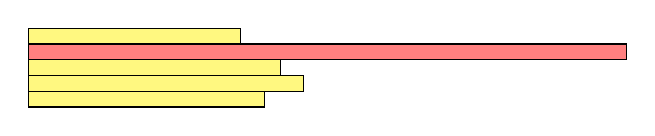
\begin{tikzpicture}[every node/.style={thick}]
    \newcommand{\x}{0.2}

    \fill[color=yellow!50,draw=black] (0,0*\x) rectangle (3,1*\x);
    \fill[color=yellow!50,draw=black] (0,1*\x) rectangle (3.5,2*\x);
    \fill[color=yellow!50,draw=black] (0,2*\x) rectangle (3.2,3*\x);
    \fill[color=red!50,draw=black] (0,3*\x) rectangle (7.6,4*\x);
    \fill[color=yellow!50,draw=black] (0,4*\x) rectangle (2.7,5*\x);
\end{tikzpicture}
\end{document}